\newpage
\section{Testy}

Dobrą praktyką pozwalającą znacznie ograniczyć występowanie błędów w ostatecznej 
wersji systemu jest przygotowanie testów sprawdzających działanie poszczególnych 
funkcji. Istnieją kilka rodzajów testów, które można pogrupować tak jak na rysunku
\ref{fig:test-types}.

\begin{figure}[h]
    \centering
    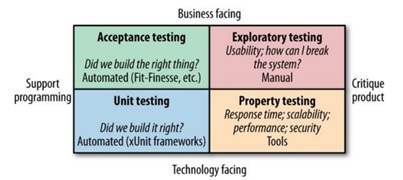
\includegraphics[width=1\textwidth]{test_types.jpg}
    \caption{Rodzaje testów. Źródło: \cite{newman2015}}
    \label{fig:test-types}
\end{figure}

Dwie kategorie znajdujące się na dole - unit testing oraz property testing - mają 
pomóc deweloperom stworzenie działającego kodu. Tego rodzaju testy mają na celu 
sprawdzenie, czy system nie jest obciążony usterkami związanymi z implementacją. 
Celem testów należących do dwóch kategorii znajdujących się na górze - acceptance 
testing oraz exploratory testing - jest pomoc w zrozumieniu jak dany system działa. 
Do tego rodzaju testów można zaliczyć m. in. szerokie testy obejmujące działanie dużej 
ilości serwisów, sprawdzenie funkcjonalności systemu oraz tzw. „user acceptance 
testing”, czyli testy przeprowadzone przez klienta, który zlecił budowę systemu.

\subsection{Testy jednostkowe}

Tego rodzaju testy sprawdzają poprawność pojedynczej funkcji w kodzie. Nie uruchamia 
się całego serwisu, a jedynie sprawdza jego część. Wszystkie parametry, które 
przyjmuje dana funkcja, są tworzone w trakcie testu. Testy jednostkowe są wykonywane 
w pierwszej fazie testów ze względu na szybkość ich wykonania. Ich celem jest wykrycie 
błędów związanych z daną technologią, nie zaś sprawdzenie, czy działanie systemu jest 
zgodne z oczekiwaniami klienta. Należy zapewnić dużą liczbę testów 
jednostkowych, ponieważ jest to najszybszy sposób zlokalizowania potencjalnych awarii.

Przykładem jest poniższy test:

\begin{lstlisting}
    [Test]
    public void MeasurementsTooHighIndicatorsTest()
    {
        // Arrange
        var currentMeasurement = 
        CreateMeasurementSentEvent();
        var policy = TestPoliciesDataService
            .CreateNewRoomPolicyDto(
                15, 80, 0.3f, 2, 20, 0.1f);

        // Run
        var result = 
        _policyEvaluator!
            .Evaluate(currentMeasurement, policy);
        
        // Assert
        Assert.AreEqual(
            result.TemperatureStatus, 
            EvaluatorResult.TooHigh);
        Assert.AreEqual(
            result.IlluminanceStatus, 
            EvaluatorResult.TooHigh);
        Assert.AreEqual(
            result.HumidityStatus, EvaluatorResult.TooHigh);
    }
\end{lstlisting}

Sprawdza on działanie logiki odpowiedzialnej za porównanie aktualnie panujących 
warunków w pomieszczeniu z warunkami oczekiwanymi. Test składa się z trzech części:

\begin{itemize} % lista nienumerowana
    \item Arrange - przygotowanie niezbędnych komponentów potrzebnych do przetestowania 
    fragmentu kodu
    \item Run - faktyczne uruchomienie testowanego kodu
    \item Assert - sprawdzenie otrzymanego wyniku z oczekiwanym rezultatem
\end{itemize}

\subsection{Testy integracyjne}

Testy integracyjne mają na celu sprawdzenie, czy poszczególne mikroserwisy będą 
w stanie się ze sobą skutecznie komunikować. Przykładem jest poniższy test:

\begin{lstlisting}
    [Test]
    public async Task 
    GetExpectedRoomConditionsAvailabilityTest()
    {
        var path = 
        $"policies-api/expected-room-conditions/1";
    
        var response = await _client.GetAsync(path);
    
        response.StatusCode.Should().Be(HttpStatusCode.OK);
    }    
\end{lstlisting}

Klient testowy korzysta z oferowanego przez testowany mikroserwis styku poprzez 
wysłanie żądania http. W tym przypadku nie jest testowana logika zawarta w testowanym 
mikroserwisie, a jedynie odpowiedź, którą odsyła. Status odpowiedzi powinien oznaczać 
sukces, sygnalizowany przez kod 200 OK \cite{fielding1999}.

\subsection{Testy end-2-end}

Testy typu end2-end mają za zadanie przetestować pewne biznesowe 
funkcjonalności, których realizacja może być obsługiwana przez wiele mikroserwisów. 
Dobrą praktyką jest utrzymywanie niewielkiej liczbę tego typu testów, ponieważ 
obejmują one zakres całego systemu i przeprowadzenie każdego z nich zajmuje dużo 
czasu. Ponadto, w przypadku wystąpienia usterki ciężko jest wykryć miejsce, które 
było źródłem błędu.
Przykładem jest poniższy test:

\begin{lstlisting}
def measurement_triggers_policies_evaluation_result_event():
    new_measurement_test_helper = NewMeasurementTestHelper()

    # check that influxdb is available and bucket exists
    new_measurement_test_helper
        .check_influxdb_is_available()

    # check that sensors_api is available
    new_measurement_test_helper
        .check_sensors_api_is_available()

    # send new measurement to rabbitmq
    new_measurement_test_helper
        .send_new_measurement_to_rabbitmq()

    # check that new measurement has 
    been sent to sensors test queue
    new_measurement_test_helper
    .check_message_sent_to_queue(
        new_measurement_test_helper
        .rabbitmq_configuration.vhost,
        consts.sensors_test_queue, 
        1)

    # check that MeasurementSentEvent has 
    been sent to test queue  
    new_measurement_test_helper.
    check_message_sent_to_queue(
        new_measurement_test_helper
        .rabbitmq_configuration.vhost,
        consts.measurement_sent_event_test_queue, 
        1)

    # check that PoliciesEvaluationResultEvent has 
    been sent to test queue
    new_measurement_test_helper.
    check_message_sent_to_queue(
        new_measurement_test_helper
        .rabbitmq_configuration.vhost,
        consts.policies_evaluation_result_event_test_queue, 
        1)


\end{lstlisting}

W tym teście sprawdza się odpowiedź całego systemu na otrzymanie nowego pomiaru 
z sensora. Jako skutek powinna zostać wygenerowana odpowiednia wiadomość z wynikiem 
przetworzenia pomiaru na kolejce wiadomości.

\subsection{Automatyzacja testów}

Ręczne uruchamianie każdego z testów pojedynczo może szybko stać się żmudnym zajęciem. 
Aby temu zaradzić, w ramach pracy inżynierskiej wykorzystano narzędzie do automatyzacji 
o nazwie Nuke \cite{nuke2022}. 
Za jego pomocą uruchomienie wszystkich testów sprowadza się do wykonania 
jednej komendy. 

Nuke pozwala na tworzenie własnych metod zwanych targetami, które automatyzują 
wykonywanie pewnych czynności. Każdy z targetów wykonują określoną logikę. 
Dodatkowo, można tworzyć kompleksową strukturę, w której każdy z targetów jest zależny 
od tego, czy prawidłowo zostanie wykonany inny target. Istnieje także możliwość 
dodania reguły wyzwalania poszczególnych targetów po wykonaniu innego. 
Przykładowo, metoda uruchamiająca test dla konkretnego projektu wygląda w sposób 
następujący:

\begin{lstlisting}
Target TestProject => _ => _
.DependsOn(CompileTestProject)
.Executes(() =>
{
    var solution = (this as IHaveSolution).Solution;
    var project = solution
        .AllProjects
        .Single(x => 
        x.Name == TestProjectNames[ProjectName]);
    DotNet($"test {project} --no-build -c {Configuration}");
});
\end{lstlisting}

Wykonuje ona metodę dotnet test, uruchamianą dla projektu o nazwie ProjectName. 
Target zależy od innej metody o nazwie CompileTestProject.

\begin{lstlisting}
Target CompileTestProject => _ => _
.DependsOn(RestoreTestProject)
.Executes(() =>
{
    var solution = (this as IHaveSolution).Solution;
    var project = solution
        .AllProjects
        .Single(x => 
        x.Name == TestProjectNames[ProjectName]);
    DotNetBuild(s => s
        .EnsureNotNull(
            this as IHaveSolution, (_, o) => 
            s.SetProjectFile(project))
        .SetConfiguration(Configuration)
        .EnableNoRestore());
});
\end{lstlisting}

Metoda wykonuję komenę dotnet build dla projektu o nazwie ProjectName. Jest ona 
zależna od targetu RestoreTestProject.

\begin{lstlisting}
Target RestoreTestProject => _ => _
.DependsOn(Clean)
.Requires(() => ProjectName)
.Executes(() =>
{
    var solution = (this as IHaveSolution).Solution;
    foreach (var proj in solution.AllProjects)
    {
        Logger.Info(proj.Name);
    }
    var project = solution
        .AllProjects
        .Single(x => 
        x.Name == TestProjectNames[ProjectName]);
    DotNetRestore(s => 
    s.EnsureNotNull(
        this as IHaveSolution, (_, o) => 
        s.SetProjectFile(project)));
});
\end{lstlisting}

Metoda wykonuje funkcję dotnet restore na projekcie o nazwie ProjectName. Jednym z 
warunków uruchomienia tego targetu jest konieczność podania nazwy projektu, wyrażona 
przez funkcję .Requires(() => ProjectName). Target jest zależny od innego targetu o 
nazwie Clean.

\begin{lstlisting}
Target Clean => _ => _
.Executes(() =>
{
    SourceDirectory
    .GlobDirectories("**/bin", "**/obj")
    .ForEach(DeleteDirectory);
    EnsureCleanDirectory(ArtifactsDirectory);
});
\end{lstlisting}

Metoda czyści repozytorium z artefaktów. Nie jest zależna od żadnego innego targetu.
Wszystkie targety można uruchomić przy wykorzystaniu tylko jednej metody:

\begin{lstlisting}
./build.sh TestProject --ProjectName facilities 
    --verbosity verbose
\end{lstlisting}